\chapter{Optische Geräte}
Bei diesem Versuch soll selbständig mit einfachen, aber grundsätzlich wichtigen optischen Geräten experimentiert werden. Im Vordergrund steht hier also das eigene Beobachten. Die quantitative Auswertung beruht auf den Gesetzten der geometrischen Optik. Konkret lässt sich dies an folgenden Aufgaben festmachen:
\begin{itemize}
 \item  Theoretische Überlegungen und Berechnungen experimentell überprüfen
 \item Grundgesetze der geometrischen Optik durch Anwenden besser verstehen
 \item  Probleme der geometrischen Optik praktisch lösen
 \item  Versuchsaufbauten justieren und optimieren
 \item Wichtige optische Geräte und Instrumente (Lupe, Fernrohre, Projektionsapparat, Mikroskop)
 in offener Versuchsanordnung nachbauen
\end{itemize}
Es wird mit folgenden Geräten experimentiert:
\begin{itemize}
 \item Lupe: Konvexlinse, die ein vergrößertes virtuelles Bild des Gegenstandes erzeugt, der sich innerhalb der Brennweite befindet
 \item Astronomisches Fernrohr: (auch Keplersches Fernrhr genannt) besteht aus zwei Sammellinsen
 \item Terrestrisches Fernrohr: besteht aus drei Linsen, wobei die Zwischenlinse der Bildumkehr dient
 \item Das holländische Fernrohr (Galileiisches Fernroht): aufgebaut aus Sammel- und Zerstreuungslinse
 \item Diaprojektor: aufgebaut aus Lampe, Kondensator, Objektiv und Schirm
 \item Erzeugung eines vergrößerten, auf dem Kopf stehenden, seitengedrehten Bild
 \item zwei Strahlengänge: beleuchtend und abbildend
 \item Mikroskop: Entwerfung eines reelen Zwischenbildes in vergößertem Maßstab, welches mit einer Lupe beobachtet wird
\end{itemize}
\newpage
\section{Fragen zur Vorbereitung}
1. Wie lautet die Abbildungsgleichung für dünne Sammel- und Zerstreuungslinsen? Welche Näherungen werden bei der Herleitung gemacht? Was ist die Hauptebene einer Linse?\\
Abbildungsgleichung für dünne Linsen:   $\frac{1}{b}+\frac{1}{g}=\frac{1}{f}=(n-1)\left(\frac{1}{r_1-r_2}\right)$ falls $d \ll r_1, r_2$\\
g= Gegenstandsweite \\
b= Bildweite\\
f= Brennweite\\ \\
Hauptebene: zwei in einem Abbildungssystem definierte Ebenen, in denen vereinfacht die Brechungen der Lichtstraheln angenommen werdenm im Raum zwischen den Hauptebenen werden die Lichtstrahlen parallel zur optischen Achse verlaufend gedacht\\
2. Wodurch werden die Bildhelligkeit und das Gesichtsfeld beeinflusst bzw. begrenzt?\\
Gesichtsfeld = allle zentralen peripheren Gegenstände und Punkte des Außenraums, die bei ruhiger, gerader Kopfhaltung und geradeaus gerichteten, bewegungslosem Blick wahrgenommen werden können, auch ohne sie direkt zu fixieren\\
Umfang des Gesichtsfeldes ist abhängig von der Pupillenweite und der Lage des Auges zu den Nachbarorganen (Nase, Augenlid). Bei teif in der Augenhöhle sitzenden Augen ist das Gesichtsfeld kleiner. An der Innenseite ist die größte Ausdehnung, an der Innenseite die kleinste. Die Farbenempfindlichkeit ist nicht an allen Stellen gleich - die äußerste Peripherie des Gesichtsfeldes ist die "farbenlose Zone", nach der Mitte zu folgt des Gesichtsfeld von blau, gelb, rot und grün. \\
Bildhelligkeit = Beleuchtungsstärke in der Bildebene eines abbildenden Systems oder Grauwert (digitales Bild)
Bild wird heller, je größer der Linsendurchmesser ist, d.h. je mehr von der Strahlungsenergie einfangen werden kann. \\\\
3. Leiten Sie die Formeln für die Vergrößerung von Lupe, den Fernrohren und dem Mikroskop
her. Berücksichtigen Sie beim Fernrohr insbesondere die großen Gegenstandsweiten.\\
Allgemein gilt:
\begin{align*}
%\begin{center}
V=\frac{\text{Sehwinkel mit Instrument}}{\text{Sehwinkel ohne Instrument}}=
\frac{\text{Sehwinkel mit Instrument}}{\text{Sehwinkel im Abstand $S_0$}}=
\frac{\epsilon}{\epsilon_0} \\
V_{Lupe}=\frac{\epsilon}{\epsilon_0}=\frac{G}{f_l}*\frac{S_0}{G}=\frac{S_0}{f_l} \\
V_{Mikroskop}=V_{Objektiv} \cdot V_{Okular}=\frac{l \cdot S_0}{f_{Obj} \cdot f_{Oku}}\\ (l=Tubulänge)\\
V_{Fernrohr}= V_{Objektiv} \cdot V_{Okular}= \frac{\frac{B}{S_0}}{\frac{G}{g}}=\frac{f_{Objekiv}}{f_{Okular}}\\
V_{Holländisches Fernrohr}=\frac{f_{Objektiv}}{|f_{Okular}|}\\
%\end{center}
\end{align*}
\\4. In welche Entfernungsbereiche - bezogen auf die Brennweite der Lupe - können der zu betrachtende Gegenstand und das Auge gebracht werden?\\
Bei einer Lupe beträgt der ideale Abstand zum Auge 25 cm, wenn der Gegenstand im Brennpunkt liegt. Liegt der Gegenstand zwischen Brennpunkt und Linse, ist das Auge angespannt, man muss das Auge auch näher an die Linse bringen. Falls sich der Gegenstand hinter der Brennweite befindet, kann er nicht mehr vergrößert gesehen werden.\\
\\5. Warum benutzt man in der Praxis meist Prismenfernrohre? Zeichnen Sie den Strahlengang!\\
\begin{figure}[h]
 \centering
 \subfigure[Strahlengang bei Umkehrprismen] {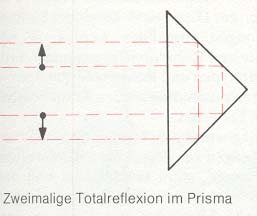
\includegraphics[width=0.49\textwidth]{prismenumkehr1}}
 % \caption{Gesichtsfeldblende und Umkehrprismen}
 \subfigure[Bildumkehr]{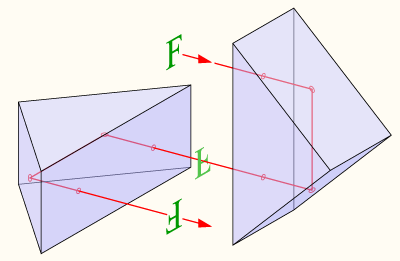
\includegraphics[width=0.49\textwidth]{prismenumkehr2}}
\end{figure}
Das Prismenfernrohr besteht wie das astronomische Fernrohr aus Obetiv und Okular. Das astronomische Fernrohr ergibt aber ein kopfstehtendes Bild. Zur Umkehrung dieses Bildes werden Prismen benutzt. Da bei dem kopfstehenden Bild auch links und rechts vertauscht werden, muss der Strahlengang noch ein zweites Prisma durchlaufen, damit auch die Seitenrichtigkeit wiederhergestellt ist. Diese Prismenanordnung bringt gegenüber dem terrestrischen Fernrohr durch den 3fach nebeneinanderglegten Strahlengang eine wesentlich verkürzte Baulänge. Der gegenüber dem Augenabstand vergrößerte Objektivabstand ist für das räumliche Sehen von Vorteil. \\ \\
6. Erläutern Sie anhand einiger einfacher optischer Abbildungsanordnungen die Begriffe Apertur und Gesichtsfeldblende. Was will man mit ihnen bezwecken?\\
\underline{Gesichtsfeldblende:} gibt der optischen Abbildung eine scharfe Begrenzung. Der abgebildete Bildausschnitt kann somit verändert werden, die Helligkeit des Bildes bleibt unbeeinflusst (im Gegensatz zur Aperturblende)  \\
\underline{Aperturblende}: begrenzt bei einem optischen System dessen Apertur (Öffnungsweite), bei Verkleinerung der Apertur werden Helligkiet und AUflösung geringer, die Schärfentiefe wird größer und der Bildausschnit bleibt erhalten (beim Auge ist die Iris die Aperturblende)
\begin{figure}[h]
\centering
 \subfigure[Gesichtsfeldblende und Umkehrprismen] {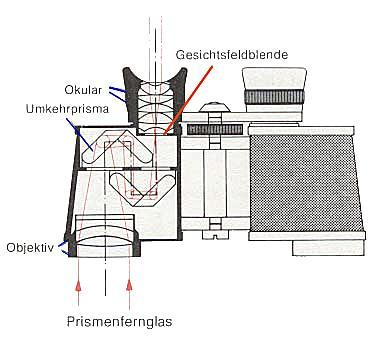
\includegraphics[width=0.49\textwidth]{gesichtsfledblende}}
% \caption{Gesichtsfeldblende und Umkehrprismen}
 \subfigure[Aperturblende]{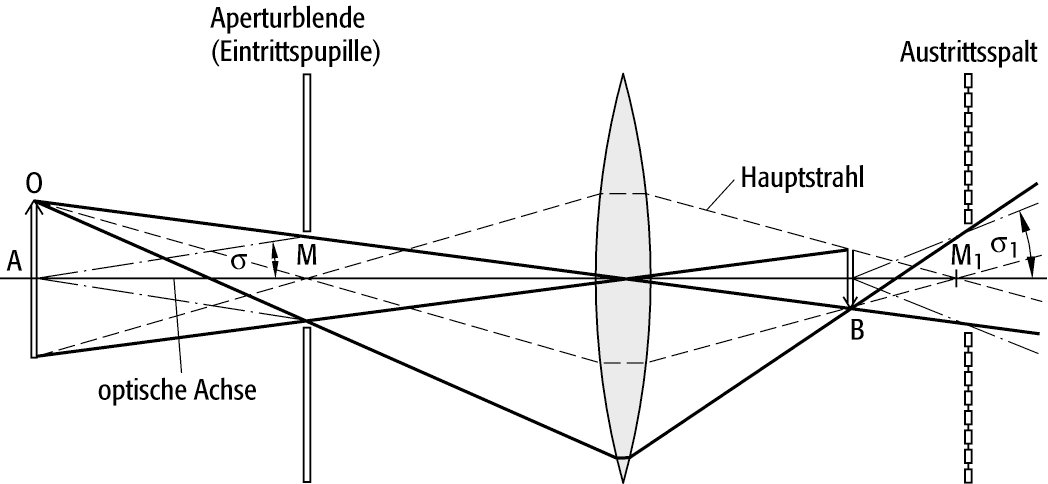
\includegraphics[width=0.49\textwidth]{Apertur}}
\end{figure}

7. Wie lassen sich in optischen Systemen mit einem vorgegebenen Linsensatz kurze Brennweiten
erzielen?\\
Es gilt: $\frac{1}{f}=\frac{1}{f_1}+\frac{1}{f_2}-\frac{d}{f_1f_2}$\\
$\rightarrow$ Kurze Brennweiten lassen sich durch einen möglichst kleinen Abstand d erzielen\\
\\8. Welche Linsenfehler gibt es? Nennen Sie Möglichkeiten zu ihrer Beseitigung!\\
\underline{sphärische Aberration:} bewirkt Unschärfe des Bildes; Beseitigung durch Unterdrückung achsenferner Strahlen mithilfe einer Blende\\
\underline{Astigmatismus:} Objekte, die außerhalb der optischen Achse liegen, werden unscharf abgebildet; Korrektur durch Kombination von sphärischen und torischen Gläsern. Die Hornhautverkrümmung kann auch operativ behandelt werden.\\
\\9. Erläutern Sie, warum Präzisionsfernrohre für die Astronomie nicht mit Linsen sondern mit
Spiegeln gebaut werden.\\
Es werden Spiegel benutzt, da sie eine größere Fläche abbilden können und billiger sind. Außerdem kann es keinen Farbfehler geben.\\\\
10. Zeichnen und erläutern Sie die Optik im menschlichen Auge! Erörtern Sie Kurz- und Weitsichtigkeit sowie Astigmatismus.\\
\begin{figure}[h]
 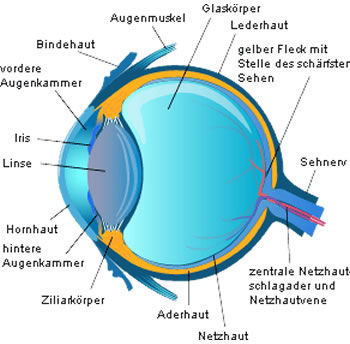
\includegraphics[width=0.5\textwidth]{Auge}
 \caption{Anatomie des Auges}
\end{figure}
Hornhaut: schützt das Auge nach außen\\
Iris und Pupille: Iris regelt Größe der Pupille und damit die Menge des durch die Linse durchtretenden Lichts\\
Linse: wesentliches Abbildungssystem des Auges\\
Glaskörper: Bestandteil des Abbildungssystems, sorgt für konst. Abstand Linse + Netzhaut\\
Netzhaut: beinhaltet Sehsinneszellen (Zäpfchen + Stäbchen)\\
Aderhaut: enthält Versorgungssystem für Netzhaut\\
Lederhaut: schützt das Auge nach außen
\underline{Kurzsichtigkeit:} zu langer Augapfel, der Fokus liegt vor der Netzhaut\\
\underline{Weitsichtigkeit:} zu kurzer Augapfel, der Fokus liegt hinter der Netzhaut\\
\underline{Astigmatismus:} siehe Aufgabe 8, Ursache: Hornhaut nicht exakt kreisförmig, sondern torisch, unterschiedliche Brechkraft an unterschiedlichen Stellen der Hornhaut, Strahlen bündeln sich nicht an einem Punkt
\\\\
11. Warum besteht der Kondensor eines Diaprojektors aus zwei plankonvexen Linsen? (Hinweis:
Berücksichtigen Sie die Reflexionsverluste!)
Plankonvexe Linsen werden benutzt, um die Dias besser auszuleuchten, ein möglichst großer Teil des Lichts der Projektionslampe soll in den abbildenden Strahlengang eingebracht werden, Verringerung der sphärischen Aberration und Totalreflexion\\
\\12. Wie kann man die Vergrößerung eines Fernrohrs ohne Kenntnis der Brennweiten messen?\\
Die Vergrößerung eines Fernrohres kann man mithilfe der Durchmesser ein- und ausfallenden Strahlenbündel bestimmen.\\
$V=\frac{d_{Aus}}{d_{Ein}}$ \\
\\13. Schätzen Sie die Größenordnung der Objektivbrennweite für einen Heimdiaprojektor ab, wenn Sie Raumgröße, Dia- und Leinwandgröße in Betracht ziehen\\
Leinwandgröße: 5m, Diagröße 5cm, Abstand zwischen linse und Dia: 10cm, Abstand zwischen LInse und Wand: 10m
Für Lupe gilt: $V=\frac{B}{G} \approx\frac{5m}{5cm}=100$ \\
Für Brennweite gilt: $f=(\frac{1}{0.1m}+\frac{1}{10m})^{-1}=9.9cm$
\\
\section{Durchführung}
\subsection{Lupe}
Betrachten Sie Gegenstände mit und ohne Lupe. Bestimmen Sie bei den verschiedenen Beobach
tungsarten jeweils die subjektiv ermittelten Vergrößerungen an.
\subsection{Astronomisches Fernrohr}
Material: 2 Achromate f = 500 mm, 60 mm und f = 40 mm, 10 mm Bikonvexlinse f = 500 mm, 38
mm 2 Bikonvexlinsen f = 40 mm, = 24 mm 2 Iris-Blenden, Ständer mit Schiene und Reiter
\begin{enumerate}
 \item   Bauen Sie ein astronomisches Fernrohr von mehr als 10-facher Vergrösserung aus zwei Bikon
 vexlinsen.
 \item Benutzen Sie eine Gesichtsfeldblende. Wo muss sie stehen, damit eine Gesichtsfeldbegrenzung
 bei Betrachtung sehr weit entfernter Gegenstände entsteht?
 \item  Benutzen Sie als Objektivlinse eine achromatische Linse. Beschreiben Sie die Unterschiede in
 der Bildgüte und bestimmen Sie die Vergrösserung experimentell.
 \item Stellen Sie eine Blende vor die Objektivlinse und betrachten Sie das Bild mit verschiedenen
 Durchmessern der Blende vor dem Objektiv
 \item Benutzen Sie als Okularlinse einen Achromaten
\end{enumerate}
\subsection{Terrestrisches Fernrohr}
Bauen Sie ein terrestrisches Fernrohr gem. Abb. og.3 auf. Diskutieren Sie insbesondere die Rolle
der mittleren Linse und ihren Einfluss auf die Vergrösserung. Untersuchen Sie die Eiflusse von
Linsenqualität (Achromate) und Blenden wie beim Astronomischen Fernrohr
\subsection{Holländisches Fernrohr}
Material: Achromat f = 500 mm, Bikonkavlinse f = -100 mm Bikonkavlinse f = -200 mm, Blende,
Ständer mit Schiene und Reitern
\begin{enumerate}
 \item . Welchen Eifluss hat der Objektivdurchmesser auf den Gesichtsfelddurchmesser?
 \item Bestimmen Sie den Durchmesser des Gesichtsfeldes bei 5-facher Vergrösserung und bei 2,5
 facher Vergrösserung (in beiden Fällen gleicher Objektivdurchmesser von 32 mm). Welcher Zu
 sammenhang besteht zwischen dem Durchmesser des Gesichtsfeldes und der Vergrösserung?
 \item Bestimmen Sie in beiden Fällen die Vergrösserung experimentell.
 
\end{enumerate}
\subsection{Spiegelteleskop}
Beobachten Sie weit entfernte Gegenstände mit dem Spiegelteleskop. Beurteilen Sie Vor- und Nach
teile gegenüber den vorher gebauten Fernrohren.
\subsection{Diaprojektor}
Vorhandene Komponenten: Bikonvexlinse f = 80 mm Optische Bank Achromat f = 80 mm Lampe
Kondensor f = 130 mm Diahalter mit Diapositiv Iris-Blende Schirm
Erzeugen Sie ein vergrößertes Bild des Diapositivs auf dem Schirm.
\begin{enumerate}
 \item  Beginnen Sie ohne Kondensorlinse mit einer Bikonvexlinse als Objektiv. Bilden Sie zunächst
 möglichst scharf ab bei einer Bildgrösse von ca. 10 cm. Verschieben Sie jetzt den Schirm so,
 dass das Bild etwas unscharf wird und verkleinern Sie dann mit der Irisblende den Linsen
 durchmesser. Beschreiben Sie die beobachteten Effekte.
 \item Benutzen Sie nun bei voller Objektivöffnung den Kondensor zur Beleuchtung des Diapositives
 und beschreiben Sie die Veränderungen im Bild gegenüber Aufgabe 1.
 \item Ändern Sie wieder wie in Aufgabe 1 den Objektivdurchmesser. Beschreiben Sie die beobach
 teten Effekte.
 \item Benutzen Sie nun als Objektiv eine korrigierte Linse (Achromat) mit gleicher Brennweite unter
 Konstanthalten der Abstände. Diskutieren Sie die Bildfehler (Farbfehler, Verzerrungen, fehlen
 de Schärfentiefe).
 
\end{enumerate}
\subsection{Mikroskop}
Geräte: Lampe (mit Kondensor), Dia mit Strichgitter d = 0,1 mm halbdurchlässiger Spiegel mit Halterung, Beobachtungsschirm Okular f = 25 mm (V = 10 ), Objektiv f = 40 mm, 10 mm Berechnen Sie die optischen Parameter eines Mikroskops für die Vergrösserung V = 50. Bestimmen Sie die Vergrösserung experimentell mit Hilfe der modifizierten Mikroskopanordnung in Abb.10: Nach der Okularlinse wird eine Sammellinse L (fL = 100 mm) platziert. Ein Beobachtungsschirm S wird im Abstand der Brennweite fL aufgestellt. Durch die Wirkung dieser Sammellinse werden die parallelen Lichtbündel, die die Okularlinse unter
dem Winkel $\psi$ verlassen auf einen Punkt am Beobachtungsschirm fokussiert. Die Vergrösserung V
des Mikroskopes kann bestimmt werden aus dem Verhältnis des Winkels $\psi$
und dem Winkel, unter
dem der Gegenstand G dem ünbewaffneten Augeïm Abstand der deutlichen Sehweite, s erscheint:
\begin{center}
 $V=\frac{\psi}{arctan g/s}$
\end{center}
Als Objekt benutzen Sie am besten das Strichgitter. Um den Winkelabstand zweier Gitterlinien auf
dem Schirm zu messen, bestimmen Sie die Höhe b, die von mehreren Gitterstrichen auf dem Beob
achtungsschirm eingenommen wird, und dividieren sie durch die Zahl der Zwischenräume zwischen
den betrachteten Gitterstrichen.
